\documentclass[11pt,]{beamer}
\graphicspath{{Images/}{./}}
\usepackage{booktabs}
\usepackage{hyperref}
\usepackage{cite}
\renewcommand\citeleft{}
\renewcommand\citeright{}
\usepackage{ragged2e}
\usepackage{array}
%----------------------------------------------------------------------------------------
\usetheme{Madrid}
\usecolortheme{dolphin}
\usefonttheme{default}
\usepackage{palatino}
\usepackage[default]{opensans}
\useoutertheme{default}
%----------------------------------------------------------------------------------------
\makeatletter
\renewcommand\@biblabel[1]{}
\renewenvironment{thebibliography}[1]
     {\section*{\refname}%
      \@mkboth{\MakeUppercase\refname}{\MakeUppercase\refname}%
      \list{}%
           {\leftmargin0pt
           \advance\leftmargin2em
           \setlength\itemindent{-2em}
            \@openbib@code
            \usecounter{enumiv}}%
      \sloppy
      \clubpenalty4000
      \@clubpenalty \clubpenalty
      \widowpenalty4000%
      \sfcode`\.\@m}
     {\def\@noitemerr
       {\@latex@warning{Empty `thebibliography' environment}}%
      \endlist}
\makeatother
%----------------------------------------------------------------------------------------
\newcommand*{\eqcite}[1]{%
  \vadjust{%
    \medskip
    \scriptsize
    \hbox to \linewidth{\hfill\textit{\cite{#1}}}%
  }%
}
%----------------------------------------------------------------------------------------
\newenvironment{conditions}
  {\par\vspace{\abovedisplayskip}\noindent\begin{tabular}{>{$}l<{$} @{${}={}$} l}}
  {\end{tabular}\par\vspace{\belowdisplayskip}}
%----------------------------------------------------------------------------------------
\AtBeginSection[]{
  \begin{frame}
  \vfill
  \centering
  \begin{beamercolorbox}[sep=8pt,center,shadow=true,rounded=true]{title}
    \usebeamerfont{title}\insertsectionhead\par%
  \end{beamercolorbox}
  \vfill
  \end{frame}
}
%----------------------------------------------------------------------------------------
\hypersetup{
colorlinks=true,
    linkcolor=black,
    filecolor=magenta,      
    urlcolor=black,
}
%----------------------------------------------------------------------------------------
\title[Currency risks CH residents]{Currency risks for Swiss residents}
%\subtitle{Digital Tool for Finance}
\author[Meier \and Merki \and Thimóteo]{\href{mailto:thomaswilhelm.meier@uzh.ch}{Thomas Meier} \and \href{mailto:ivo.merki@uzh.ch}{Ivo Merki} \and \href{mailto:mateus.siqueirathimoteo@uzh.ch}{Mateus Thimóteo}}
\institute[UZH]{University of Zurich \\ \smallskip}
\date[December 22, 2023]{Presentation Digital Tools for Finance \\ \smallskip {\footnotesize December 22, 2023}}
%----------------------------------------------------------------------------------------
\begin{document}
%----------------------------------------------------------------------------------------
\begin{frame}
	\titlepage
\end{frame}
%----------------------------------------------------------------------------------------
\begin{frame}
	\frametitle{Presentation Overview}
    \tableofcontents 
\end{frame}
%----------------------------------------------------------------------------------------
\section{Introduction}
\subsection{Motivation}
\subsection{Safe haven currencies}
\subsection{Research question}
%----------------------------------------------------------------------------------------
\begin{frame}
	\frametitle{Motivation}
	\begin{figure}
		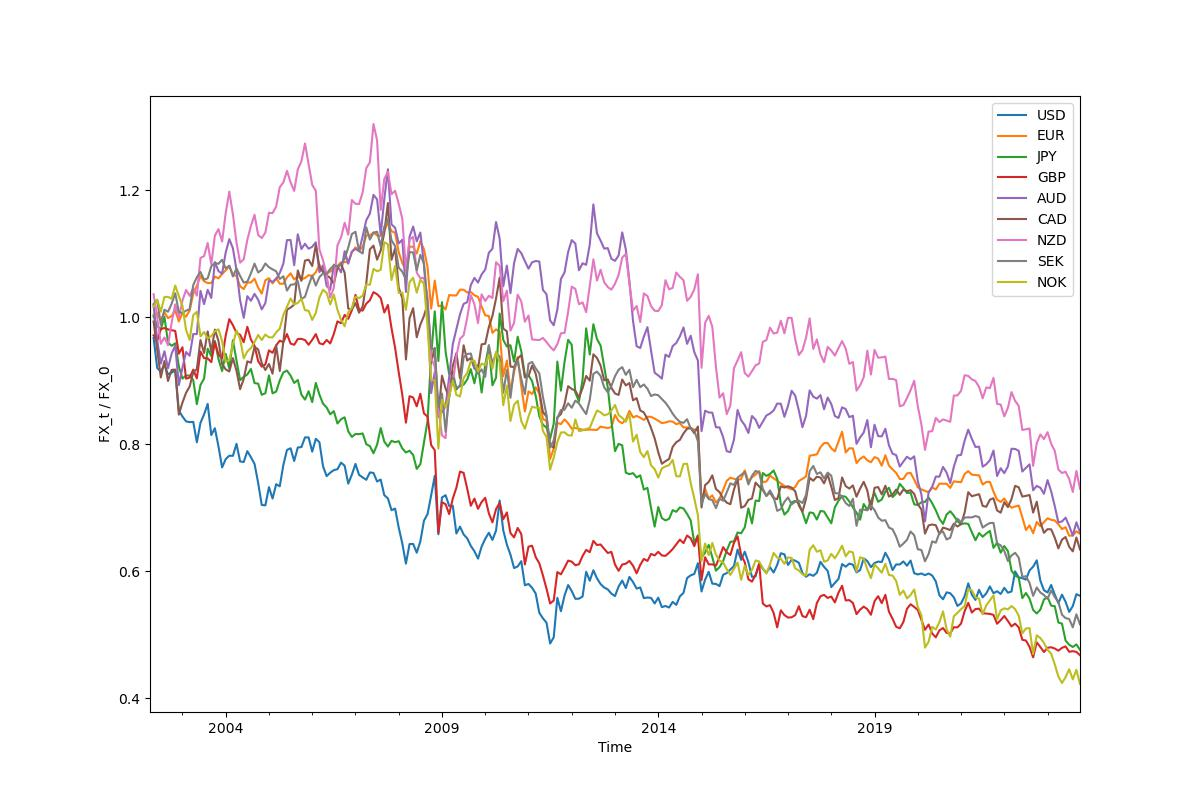
\includegraphics[width=0.8\linewidth]{figures/ccy_perfs.jpg}
		\caption{Returns in different currencies}
	\end{figure}
\end{frame}
%----------------------------------------------------------------------------------------
\begin{frame}
    \frametitle{Safe haven currencies}
    \begin{itemize}
    \setlength\itemsep{2em}
    \item Safe haven characteristics by \cite{Habib and Stracca 2012}
    \item Implications for residents of safe haven currency countries 
    \item CHF a safe haven currency
    \end{itemize}
\end{frame}
%----------------------------------------------------------------------------------------
\begin{frame}
	\frametitle{Research question}
	\bigskip
	\begin{quote}
    {\Large Which of the G10 currencies is the riskiest to hold for a Swiss resident?}
	\end{quote}
	\bigskip
\end{frame}
%----------------------------------------------------------------------------------------
\section{Analysis}
\subsection{Data}
\subsection{Model}
\subsection{Results}
%----------------------------------------------------------------------------------------
\begin{frame}[t]
	\frametitle{Data}
 \begin{itemize}
 \item \href{https://fred.stlouisfed.org/graph/?g=1cwRm}{USD/CHF Spot Exchange Rate from FRED} 
 \item \href{https://fred.stlouisfed.org/graph/?g=1cwLK}{EUR/USD Spot Exchange Rate from FRED}
 \item \href{https://fred.stlouisfed.org/graph/?g=1cwNJ}{USD/JPY Spot Exchange Rate from FRED}
 \item \href{https://fred.stlouisfed.org/graph/?g=1cwOd}{GBP/USD Spot Exchange Rate from FRED}
 \item \href{https://fred.stlouisfed.org/graph/?g=1cwOA}{AUD/USD Spot Exchange Rate from FRED}
 \item \href{https://fred.stlouisfed.org/graph/?g=1cwOW}{USD/CAD Spot Exchange Rate from FRED}
 \item \href{https://fred.stlouisfed.org/graph/?g=1cwPf}{NZD/USD Spot Exchange Rate from FRED}
 \item \href{https://fred.stlouisfed.org/graph/?g=1cwPD}{USD/SEK Spot Exchange Rate from FRED}
 \item \href{https://fred.stlouisfed.org/graph/?g=1cwPN}{USD/NOK Spot Exchange Rate from FRED}
 \item \href{https://fred.stlouisfed.org/graph/?g=1cwPY}{VIX from FRED}
 \item \href{https://data.oecd.org/chart/7hSF}{Short-term Interest Rates from OECD}
 \end{itemize}
\end{frame} 
%----------------------------------------------------------------------------------------
\begin{frame}
	\frametitle{Model}

	\begin{equation}
		\Delta s_{t+1}^k=\alpha^k+\beta_{0}^k(f_{t}^k-s_{t}^k)+\beta_{1}^k AFX_{t+1}+\beta_{2}^k\Delta VIX_{t+1}+\epsilon_{t+1}^k
	    \eqcite{Grisse and Nitschka 2015}
    \end{equation}

    \medskip
    \begin{center}
    \begin{conditions}
    $\Delta s_{t+1}^k$ & change log spot exchange rates of currencies\\    
    $f_{t}^k$ & log forward exchange rate\\    
    $AFX_{t+1}$ & average CHF exchange rate changes\\    
    $\Delta VIX_{t+1}$ & log changes VIX\\      
    \end{conditions}
    \end{center}
\end{frame}
%----------------------------------------------------------------------------------------
\begin{frame}
	\frametitle{Results}
	\framesubtitle{EUR \ USD \ JPY}
    \begin{center}
    \scalebox{0.45}{%
    \renewenvironment{table}[1][]{\ignorespaces}{\unskip}%
    
% Table created by stargazer v.5.2.3 by Marek Hlavac, Social Policy Institute. E-mail: marek.hlavac at gmail.com
% Date and time: Sun, Dec 10, 2023 - 23:55:29
% Requires LaTeX packages: dcolumn 
\begin{table}[!htbp] \centering 
  \caption{} 
  \label{} 
\begin{tabular}{@{\extracolsep{5pt}}lD{.}{.}{-3} D{.}{.}{-3} D{.}{.}{-3} } 
\\[-1.8ex]\hline 
\hline \\[-1.8ex] 
 & \multicolumn{3}{c}{\textit{Dependent variable:}} \\ 
\cline{2-4} 
\\[-1.8ex] & \multicolumn{1}{c}{EUR\_} & \multicolumn{1}{c}{USD\_} & \multicolumn{1}{c}{JPY\_} \\ 
\\[-1.8ex] & \multicolumn{1}{c}{(1)} & \multicolumn{1}{c}{(2)} & \multicolumn{1}{c}{(3)}\\ 
\hline \\[-1.8ex] 
 F\_S\_EUR & -1.598 &  &  \\ 
  & (1.218) &  &  \\ 
  & & & \\ 
 F\_S\_USD &  & -0.728 &  \\ 
  &  & (1.403) &  \\ 
  & & & \\ 
 F\_S\_JPY &  &  & -2.176 \\ 
  &  &  & (2.495) \\ 
  & & & \\ 
 delta\_Log\_VIX & -0.002 & 0.040^{***} & 0.053^{***} \\ 
  & (0.004) & (0.007) & (0.008) \\ 
  & & & \\ 
 AFX\_EUR & -0.640^{***} &  &  \\ 
  & (0.042) &  &  \\ 
  & & & \\ 
 AFX\_USD &  & -0.906^{***} &  \\ 
  &  & (0.073) &  \\ 
  & & & \\ 
 AFX\_JPY &  &  & -0.557^{***} \\ 
  &  &  & (0.085) \\ 
  & & & \\ 
 Constant & -0.002 & -0.001 & -0.002 \\ 
  & (0.001) & (0.002) & (0.002) \\ 
  & & & \\ 
\hline \\[-1.8ex] 
Observations & \multicolumn{1}{c}{258} & \multicolumn{1}{c}{257} & \multicolumn{1}{c}{258} \\ 
R$^{2}$ & \multicolumn{1}{c}{0.496} & \multicolumn{1}{c}{0.392} & \multicolumn{1}{c}{0.215} \\ 
Adjusted R$^{2}$ & \multicolumn{1}{c}{0.490} & \multicolumn{1}{c}{0.385} & \multicolumn{1}{c}{0.205} \\ 
Residual Std. Error & \multicolumn{1}{c}{0.013 (df = 254)} & \multicolumn{1}{c}{0.022 (df = 253)} & \multicolumn{1}{c}{0.026 (df = 254)} \\ 
F Statistic & \multicolumn{1}{c}{83.310$^{***}$ (df = 3; 254)} & \multicolumn{1}{c}{54.480$^{***}$ (df = 3; 253)} & \multicolumn{1}{c}{23.147$^{***}$ (df = 3; 254)} \\ 
\hline 
\hline \\[-1.8ex] 
\textit{Note:}  & \multicolumn{3}{r}{$^{*}$p$<$0.1; $^{**}$p$<$0.05; $^{***}$p$<$0.01} \\ 
\end{tabular} 
\end{table} 
%
    \unskip}
    \end{center}
\end{frame}
%----------------------------------------------------------------------------------------
\begin{frame}
	\frametitle{Results}
	\framesubtitle{GBP \ AUD \ CAD}
    \begin{center}
	\scalebox{0.45}{%
    \renewenvironment{table}[1][]{\ignorespaces}{\unskip}%
    
% Table created by stargazer v.5.2.3 by Marek Hlavac, Social Policy Institute. E-mail: marek.hlavac at gmail.com
% Date and time: Tue, Dec 19, 2023 - 21:05:04
% Requires LaTeX packages: dcolumn 
\begin{table}[!htbp] \centering 
  \caption{Regression Table GBP AUD CAD.} 
  \label{} 
\begin{tabular}{@{\extracolsep{5pt}}lD{.}{.}{-3} D{.}{.}{-3} D{.}{.}{-3} } 
\\[-1.8ex]\hline 
\hline \\[-1.8ex] 
 & \multicolumn{3}{c}{\textit{Dependent variable:}} \\ 
\cline{2-4} 
\\[-1.8ex] & \multicolumn{1}{c}{GBP\_} & \multicolumn{1}{c}{AUD\_} & \multicolumn{1}{c}{CAD\_} \\ 
\\[-1.8ex] & \multicolumn{1}{c}{(1)} & \multicolumn{1}{c}{(2)} & \multicolumn{1}{c}{(3)}\\ 
\hline \\[-1.8ex] 
 F\_S\_GBP & 0.902 &  &  \\ 
  & (1.167) &  &  \\ 
  & & & \\ 
 F\_S\_AUD &  & 0.345 &  \\ 
  &  & (1.138) &  \\ 
  & & & \\ 
 F\_S\_CAD &  &  & -0.067 \\ 
  &  &  & (1.687) \\ 
  & & & \\ 
 delta\_Log\_VIX & 0.005 & -0.038^{***} & -0.005 \\ 
  & (0.006) & (0.006) & (0.005) \\ 
  & & & \\ 
 AFX\_GBP & -0.962^{***} &  &  \\ 
  & (0.066) &  &  \\ 
  & & & \\ 
 AFX\_AUD &  & -1.075^{***} &  \\ 
  &  & (0.066) &  \\ 
  & & & \\ 
 AFX\_CAD &  &  & -1.304^{***} \\ 
  &  &  & (0.062) \\ 
  & & & \\ 
 Constant & 0.0002 & 0.001 & 0.001 \\ 
  & (0.002) & (0.003) & (0.003) \\ 
  & & & \\ 
\hline \\[-1.8ex] 
Observations & \multicolumn{1}{c}{258} & \multicolumn{1}{c}{258} & \multicolumn{1}{c}{258} \\ 
R$^{2}$ & \multicolumn{1}{c}{0.461} & \multicolumn{1}{c}{0.586} & \multicolumn{1}{c}{0.651} \\ 
Adjusted R$^{2}$ & \multicolumn{1}{c}{0.455} & \multicolumn{1}{c}{0.581} & \multicolumn{1}{c}{0.647} \\ 
Residual Std. Error (df = 254) & \multicolumn{1}{c}{0.020} & \multicolumn{1}{c}{0.020} & \multicolumn{1}{c}{0.018} \\ 
F Statistic (df = 3; 254) & \multicolumn{1}{c}{72.521$^{***}$} & \multicolumn{1}{c}{119.730$^{***}$} & \multicolumn{1}{c}{158.024$^{***}$} \\ 
\hline 
\hline \\[-1.8ex] 
\textit{Note:}  & \multicolumn{3}{r}{$^{*}$p$<$0.1; $^{**}$p$<$0.05; $^{***}$p$<$0.01} \\ 
\end{tabular} 
\end{table} 
%
    \unskip}
    \end{center}
\end{frame}
%----------------------------------------------------------------------------------------
\begin{frame}
	\frametitle{Results}
	\framesubtitle{NZD \ SEK \ NOK}
    \begin{center}
	\scalebox{0.45}{%
    \renewenvironment{table}[1][]{\ignorespaces}{\unskip}%
    
% Table created by stargazer v.5.2.3 by Marek Hlavac, Social Policy Institute. E-mail: marek.hlavac at gmail.com
% Date and time: Sun, Dec 10, 2023 - 23:17:51
% Requires LaTeX packages: dcolumn 
\begin{table}[!htbp] \centering 
  \caption{Regression Results 3} 
  \label{} 
\begin{tabular}{@{\extracolsep{5pt}}lD{.}{.}{-3} D{.}{.}{-3} D{.}{.}{-3} } 
\\[-1.8ex]\hline 
\hline \\[-1.8ex] 
 & \multicolumn{3}{c}{\textit{Dependent variable:}} \\ 
\cline{2-4} 
\\[-1.8ex] & \multicolumn{1}{c}{NZD\_} & \multicolumn{1}{c}{SEK\_} & \multicolumn{1}{c}{NOK\_} \\ 
\\[-1.8ex] & \multicolumn{1}{c}{(1)} & \multicolumn{1}{c}{(2)} & \multicolumn{1}{c}{(3)}\\ 
\hline \\[-1.8ex] 
 F\_S\_NZD & 1.395 &  &  \\ 
  & (1.149) &  &  \\ 
  & & & \\ 
 F\_S\_SEK &  & -0.319 &  \\ 
  &  & (1.530) &  \\ 
  & & & \\ 
 F\_S\_NOK &  &  & 0.710 \\ 
  &  &  & (1.479) \\ 
  & & & \\ 
 delta\_Log\_VIX & -0.038^{***} & -0.013^{**} & -0.025^{***} \\ 
  & (0.007) & (0.005) & (0.006) \\ 
  & & & \\ 
 AFX\_NZD & -0.862^{***} &  &  \\ 
  & (0.077) &  &  \\ 
  & & & \\ 
 AFX\_SEK &  & -0.795^{***} &  \\ 
  &  & (0.057) &  \\ 
  & & & \\ 
 AFX\_NOK &  &  & -0.921^{***} \\ 
  &  &  & (0.070) \\ 
  & & & \\ 
 Constant & 0.005 & -0.001 & -0.0004 \\ 
  & (0.004) & (0.002) & (0.003) \\ 
  & & & \\ 
\hline \\[-1.8ex] 
Observations & \multicolumn{1}{c}{258} & \multicolumn{1}{c}{258} & \multicolumn{1}{c}{258} \\ 
R$^{2}$ & \multicolumn{1}{c}{0.420} & \multicolumn{1}{c}{0.470} & \multicolumn{1}{c}{0.461} \\ 
Adjusted R$^{2}$ & \multicolumn{1}{c}{0.413} & \multicolumn{1}{c}{0.464} & \multicolumn{1}{c}{0.455} \\ 
Residual Std. Error (df = 254) & \multicolumn{1}{c}{0.023} & \multicolumn{1}{c}{0.017} & \multicolumn{1}{c}{0.021} \\ 
F Statistic (df = 3; 254) & \multicolumn{1}{c}{61.363$^{***}$} & \multicolumn{1}{c}{75.213$^{***}$} & \multicolumn{1}{c}{72.407$^{***}$} \\ 
\hline 
\hline \\[-1.8ex] 
\textit{Note:}  & \multicolumn{3}{r}{$^{*}$p$<$0.1; $^{**}$p$<$0.05; $^{***}$p$<$0.01} \\ 
\end{tabular} 
\end{table} 
%
    \unskip}
    \end{center}
\end{frame}
%----------------------------------------------------------------------------------------

\section{Appendix}
\subsection{References}
%----------------------------------------------------------------------------------------
\begin{frame}[t] % Use [allowframebreaks] to allow automatic splitting across slides if the content is too long
	\frametitle{References}
	\setbeamertemplate{bibliography item}{}
	\begin{thebibliography}{99}
		\footnotesize

        %\bibitem[Akram, Rime, and Sarno (2008)]{Akram and Rime and Sarno 2008}\href{https://doi.org/10.1016/j.jinteco.2008.07.004}{Akram, Q. Farooq, Dagfinn Rime, and Lucio Sarno, 2008, Arbitrage in the foreign exchange market: Turning on the microscope, pp. 237--253 in \textit{Journal of International Economics}, Vol. 76, No. 2, December.}
  
		\bibitem[Grisse and Nitschka (2015)]{Grisse and Nitschka 2015}\href{https://doi.org/10.1016/j.jempfin.2015.03.006}{Grisse, Christian, and Thomas Nitschka, 2013, On financial risk and the safe haven characteristics of Swiss franc exchange rates, pp. 153--164 in \textit{Journal of Empirical Finance}, Vol. 32, June.}
			
		\bibitem[Habib and Stracca (2012)]{Habib and Stracca 2012}\href{https://doi.org/10.1016/j.jinteco.2011.12.005}{Habib, Maurizio M., and Livio Stracca, 2012, Getting beyond carry trade: What makes a safe haven currency?, pp. 50--64 in \textit{Journal of International Economics}, Vol. 87, No. 1, May.}
 
	\end{thebibliography}
\end{frame}
%----------------------------------------------------------------------------------------
\end{document} 